% Workshop-paper skeleton (4 pages + references). Replace the preamble with the
% official ML4PS style file when the call for papers is published.
\documentclass[10pt]{article}
\usepackage[letterpaper,margin=1in]{geometry}
\usepackage{times}
\usepackage{amsmath,amssymb}
\usepackage{graphicx}
\usepackage{booktabs}
\usepackage{hyperref}
\usepackage{xcolor}
\newcommand{\todo}[1]{\textcolor{red}{[TODO: #1]}}
\newcommand{\Hbb}{\ensuremath{H\to b\bar b}}
\newcommand{\Hcc}{\ensuremath{H\to c\bar c}}

\title{Where does the Particle Transformer look for $b$ quarks?\\
Attention circuits behind heavy-flavour tagging}
\author{Avinash \\ \todo{affiliation} \\ \texttt{\todo{email}}}
\date{}

\begin{document}
\maketitle

\begin{abstract}
The Particle Transformer (ParT) is a state-of-the-art jet tagger, but it is not known what it computes internally.
We study the official pretrained ParT on JetClass and ask which mechanism separates \Hbb\ from QCD jets.
We record the content term $QK^\top/\sqrt d$ and the pairwise-interaction bias $\psi(U)$ separately in every
head, then combine attention statistics with causal interventions (head ablation, attention knockout,
activation patching) and linear probes.
\todo{one sentence per headline finding, with numbers and uncertainties.}
We compare the results with GDS-ParT, a gated variant that also uses pairwise features.
Code: \url{https://github.com/Avinashistoocool/ParT-Interpretability}.
\end{abstract}

\section{Introduction}
\todo{Jet tagging; ParT~\cite{qu2022part} and JetClass~\cite{jetclass}; interpretability work in HEP so far (top taggers~\cite{khot2023},
Lund-plane GNNs~\cite{dreyer2021}); attention is not explanation~\cite{jain2019} $\Rightarrow$ need causal tests.
Contributions: (i) an exact bias/content decomposition of ParT attention, (ii) evidence for or against a
displaced-track (``secondary-vertex'') circuit, (iii) a comparison with GDS-ParT.}

\section{Model and instrumentation}
ParT particle attention in layer $l$, head $h$:
\begin{equation}
A^{(l,h)} = \mathrm{softmax}\!\Big(\tfrac{Q^{(l,h)}K^{(l,h)\top}}{\sqrt d} + \psi_h(U) + M\Big),
\end{equation}
where $U_{ij}=(\ln\Delta_{ij},\ln k_{T,ij},\ln z_{ij},\ln m^2_{ij})$, $\psi$ is shared across layers and $M$ masks padding.
Two class-attention blocks~\cite{cait} then read the particles into a CLS token. We re-implement the forward
pass around the original weights. It reproduces the logits of the reference implementation (max deviation
\todo{x}) and exposes $QK^\top$, $\psi(U)$, $A$, head contexts and the residual stream for recording and editing.

\section{Experimental setup}
Pretrained \texttt{ParT\_full} (17 particle features, including $\tanh d_0$, $\sigma_{d_0}$)~\cite{qu2022part}. JetClass validation
files (not used in training), \todo{N} jets per class. A charged track is \emph{displaced} if $|d_0|/\sigma_{d_0}>3$.
This is a reco-level proxy for $b/c$ decay products. Uncertainties are 68\% bootstrap intervals over jets.

\section{Results}
\subsection{What the classifier reads}
\todo{Fig.~\ref{fig:cls}: CLS attention enrichment per particle category; regression coefficients.}
\begin{figure}[t]\centering
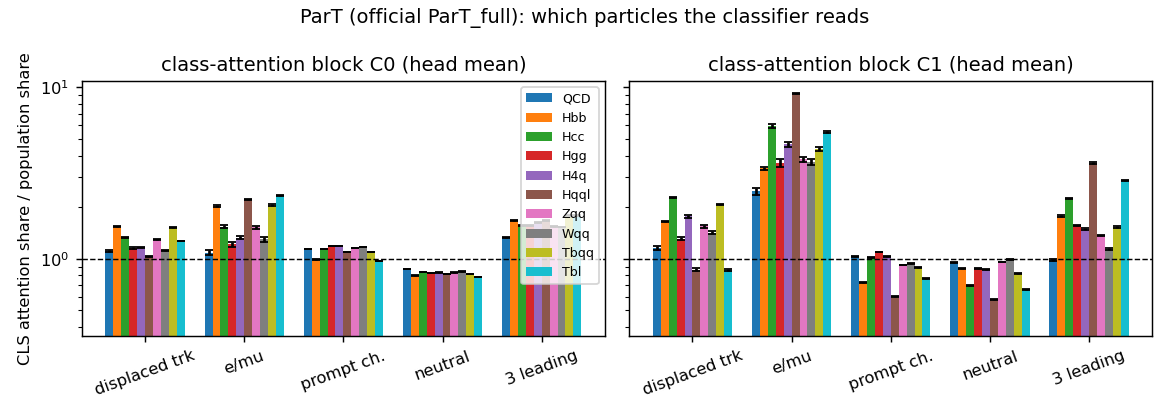
\includegraphics[width=\linewidth]{figures/fig1_cls_enrichment.png}
\caption{CLS attention share divided by population share, per particle category and jet class. \todo{caption}}
\label{fig:cls}\end{figure}

\subsection{Head specialisation and a secondary-vertex-like head}
\todo{Fig.~\ref{fig:heads}: Spearman correlation with pairwise kinematics per head; displaced$\to$displaced enrichment vs permutation null.}
\begin{figure}[t]\centering
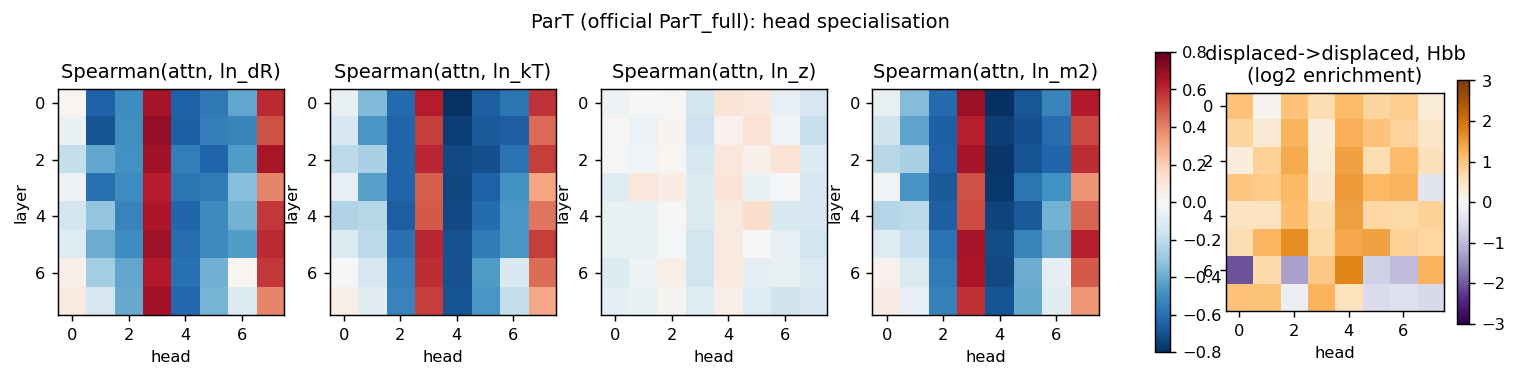
\includegraphics[width=\linewidth]{figures/fig2_head_pairwise.png}
\caption{\todo{caption}}\label{fig:heads}\end{figure}

\subsection{Interaction bias versus content}
\todo{Fig.~\ref{fig:bias}: share of logit variance from $\psi(U)$ by layer; effect of removing either term.}
\begin{figure}[t]\centering
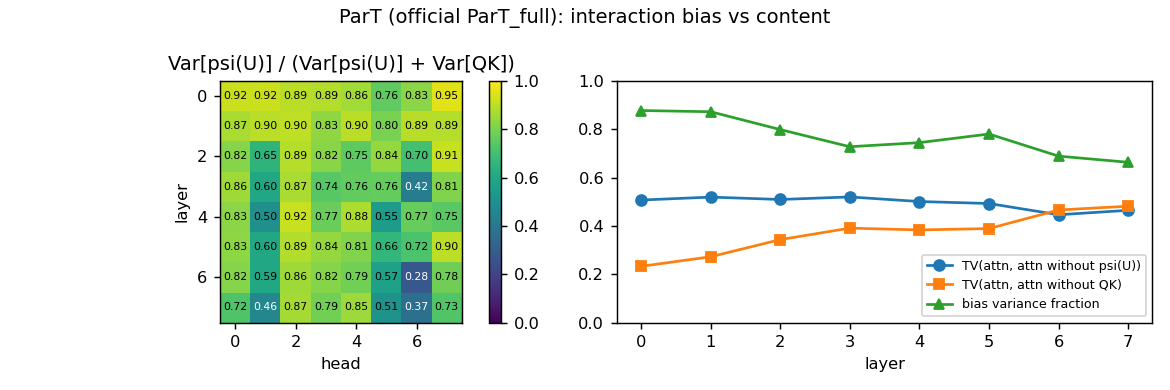
\includegraphics[width=0.8\linewidth]{figures/fig3_bias_vs_qk.png}
\caption{\todo{caption}}\label{fig:bias}\end{figure}

\subsection{Causal tests}
\todo{Table~\ref{tab:causal}: head ablation, bias removal, attention knockout (displaced vs $p_T$-matched prompt), activation patching.}
\begin{table}[t]\centering\small
\begin{tabular}{lccc}\toprule
intervention & $\Delta$AUC (\Hbb\ vs QCD) & $\Delta\,$logit (sig) & $R_{50}$ ratio \\\midrule
\todo{rows from results/REPORT\_*.md} & & & \\\bottomrule
\end{tabular}
\caption{\todo{caption}}\label{tab:causal}\end{table}

\subsection{Linear probes}
\todo{Fig.: probe AUC by depth for displaced / lepton / displaced-neighbour; random-init and shuffled-label controls~\cite{belinkov2022}.}

\subsection{Comparison with GDS-ParT}
\todo{Same analyses; differences in where displacement information is integrated.}

\section{Limitations}
Reco-level displacement proxy without truth vertex matching; Delphes simulation; attention-based measures are
correlational; patching corruptions are partly off-distribution; one pretrained seed (ParT authors release one).

\section{Conclusion}
\todo{}

\bibliographystyle{unsrt}
\bibliography{refs}
\end{document}
